\documentclass[12pt,a4paper]{article}%[a4paper,portuguese,12pt,pdftex]{article} %article
\usepackage{ucs}
\usepackage{amsfonts}		 		% usar fontes p/ REAL,IMAGINARIO,etc
\usepackage{indentfirst}			% espacamento no 1o. paragrafo
\usepackage[utf8x]{inputenc} 
\usepackage{amssymb,amsmath}			% pacote simbolos e matematico AMS
\usepackage{textcomp}
\usepackage{natbib}				% estilo de citacao no texto
\usepackage{wasysym}
\usepackage{fancyhdr}
\renewcommand{\baselinestretch}{1.5}		% espaco entre linhas
\topmargin -1cm					% margem superior
\oddsidemargin 0.5cm				% margem esquerda
\textwidth 15cm					% largura da pagina
\textheight 23.7cm				% altura da pagina
\usepackage{color}
\usepackage{lscape}
\usepackage{graphicx}
\usepackage{epsfig}

\title{Learning velocity fields from sparse data using Gaussian Process}
\author{}

\begin{document}
\section{Reconstruction of a non-divergent velocity field}
In this exercise, I applied the non-divergent kernel to reconstruct 
a non-divergent velocity field. The velocity field was created by taking 
the curl of a 2D Gaussian surface. To reconstruct this velocity field, 
20 random samples were taken as observations, and the grid of the reconstructed 
velocity field was exactly the same as the one from the original velocity field. 
No noise was added to the observations, and the observations where assumed to 
have no error.

\newpage

\begin{figure}
\noindent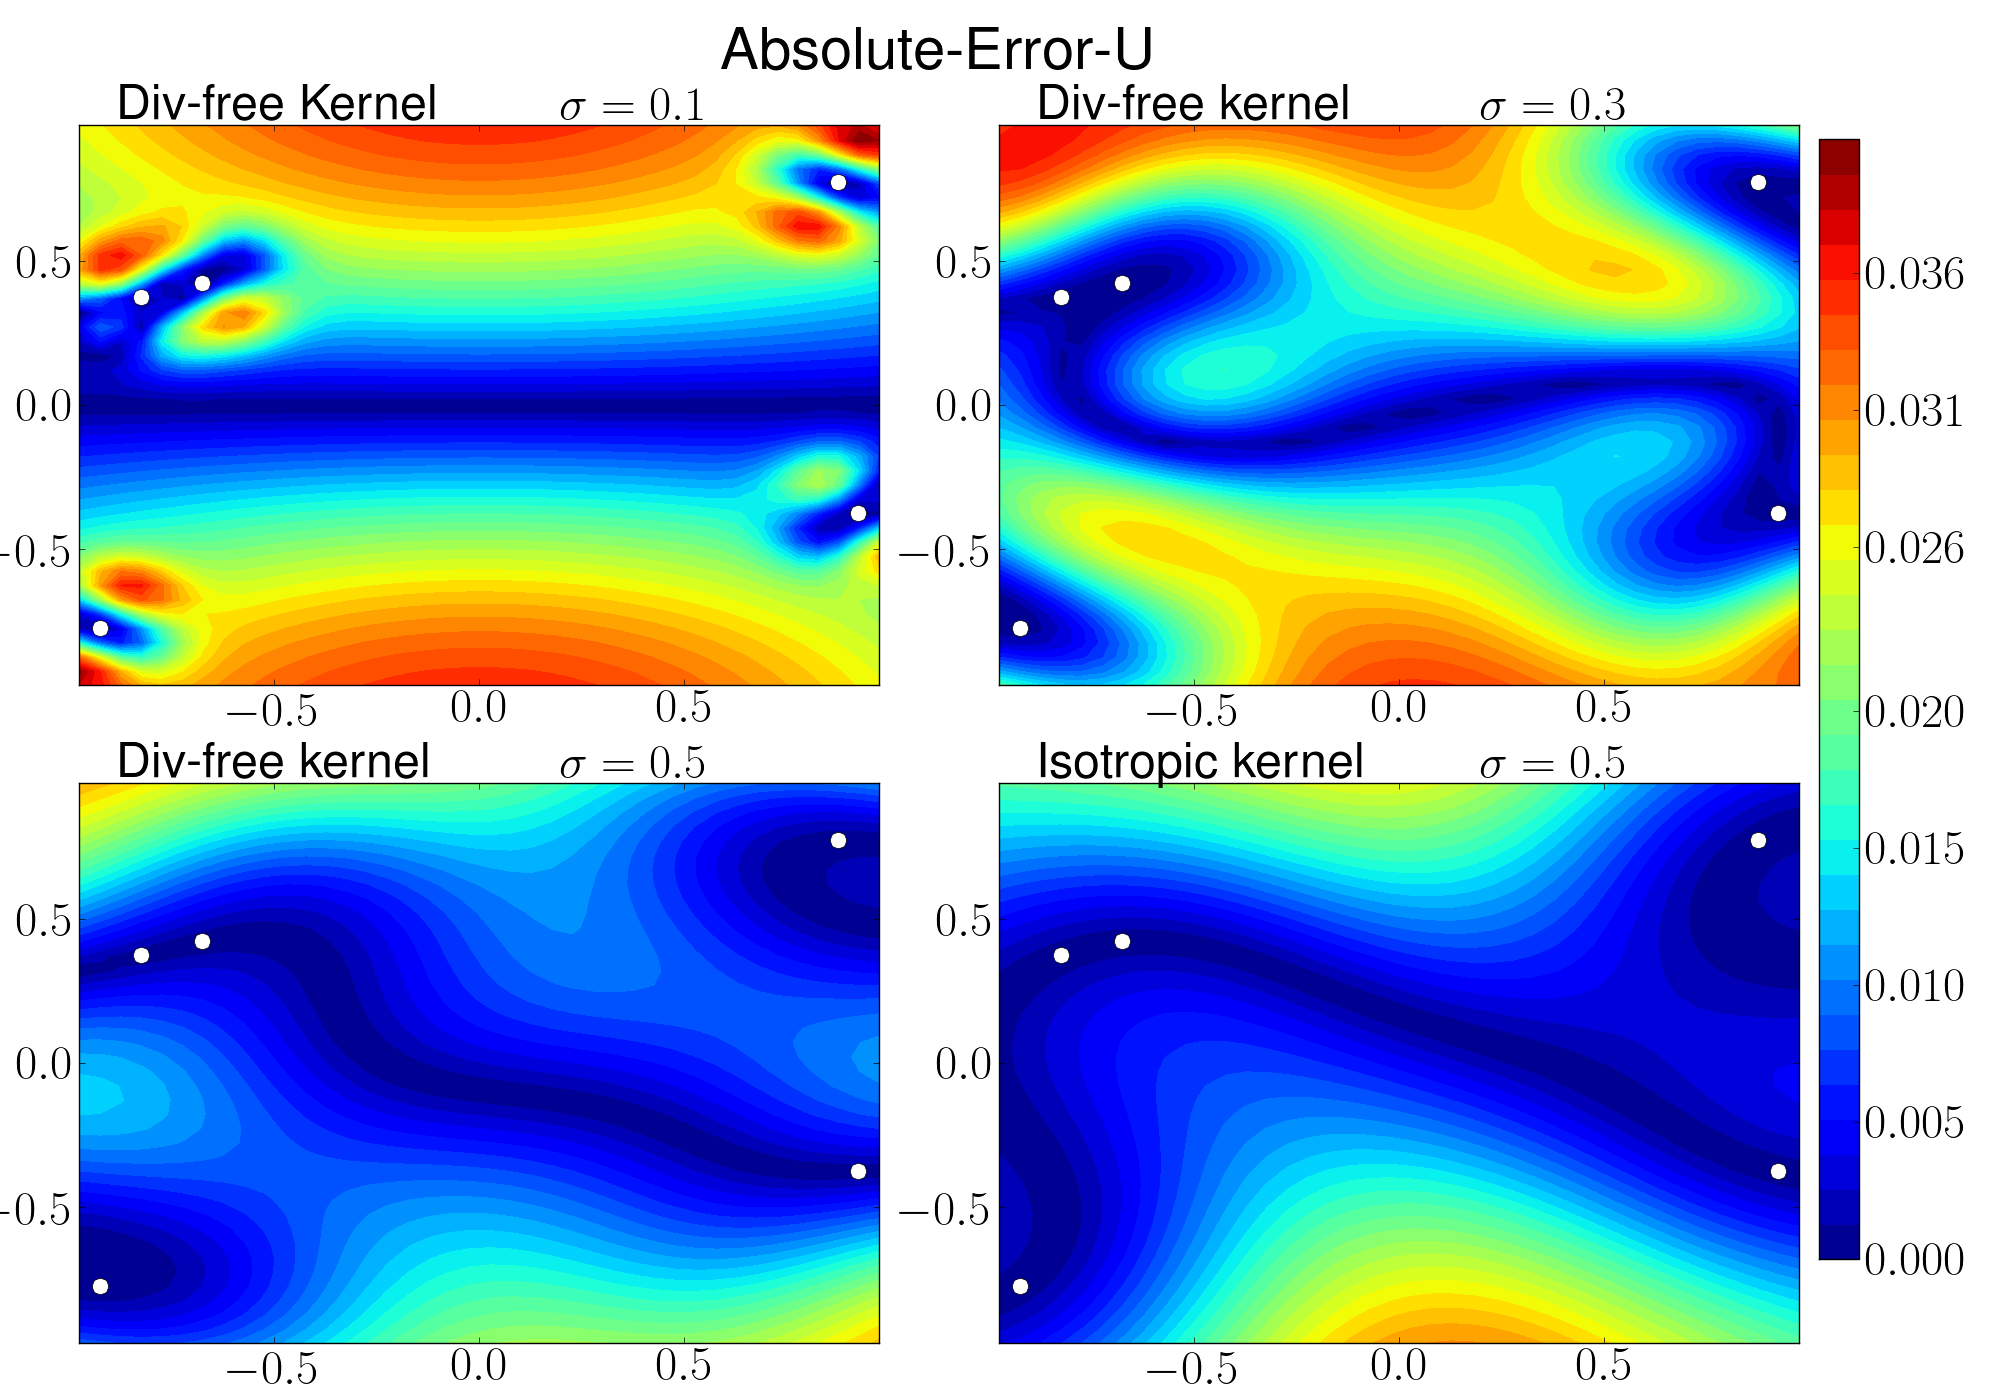
\includegraphics[width=36pc]{plots/Absolute-Error-U-contour.png}
\caption{Absolute error of the zonal velocity for 4 different cases. Top-left: 
divergence free kernel and decorrelation distance ($\sigma$) of 0.1. 
Top-right: divergence-free kernel and $\sigma=0.3$. Bottom-left: 
divergence-free kernel and $sigma=0.5$. Bottom-right: isotropic 
squared-exponential kernel and $\sigma=0.5$. The black dots indicate the location 
of the observations.}
\label{contour_u}
\end{figure}

\begin{figure}
\noindent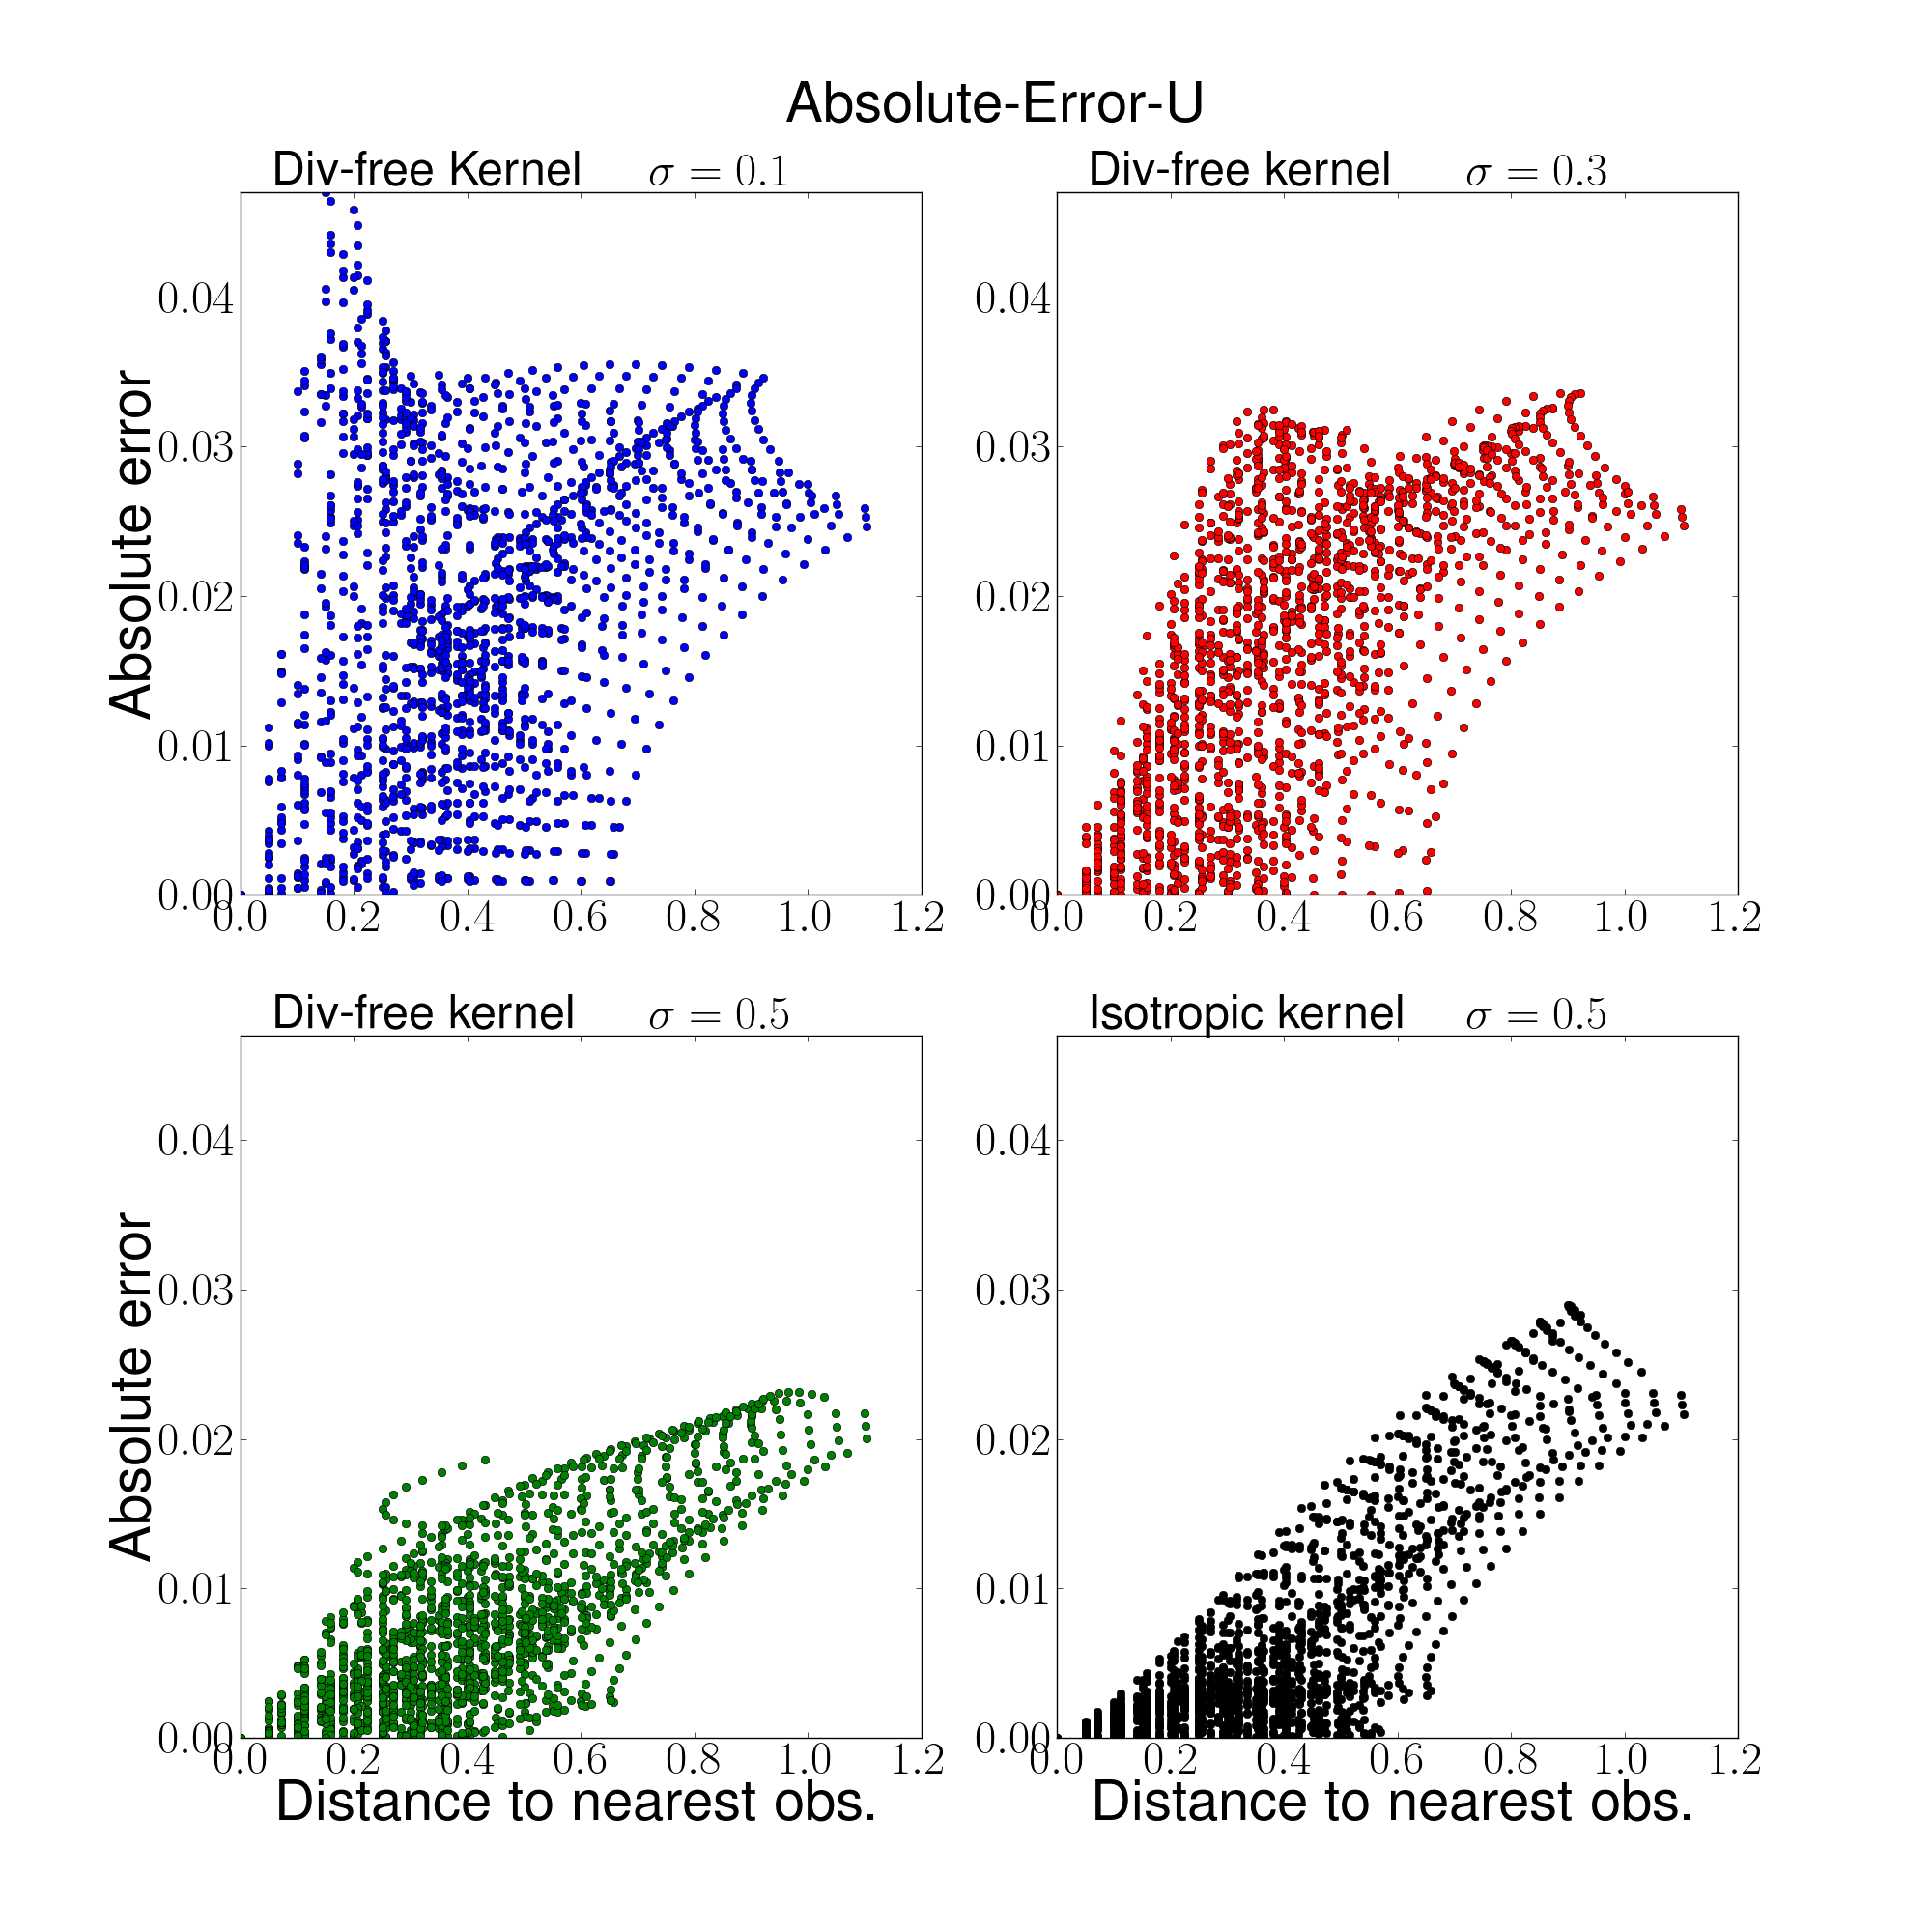
\includegraphics[width=36pc]{plots/Absolute-Error-U-scatter.png}
\caption{Scatter plots of absolute error by distance to nearest observation of 
the zonal velocity component for 4 different cases. Top-left: divergence free kernel and 
decorrelation $\sigma=0.1$. Top-right: divergence-free kernel and 
$\sigma=0.3$. Bottom-left: divergence-free kernel and $sigma=0.5$. Bottom-right: isotropic 
squared-exponential kernel and $\sigma=0.5$.}
\label{scatter_u}
\end{figure}


\begin{figure}
\noindent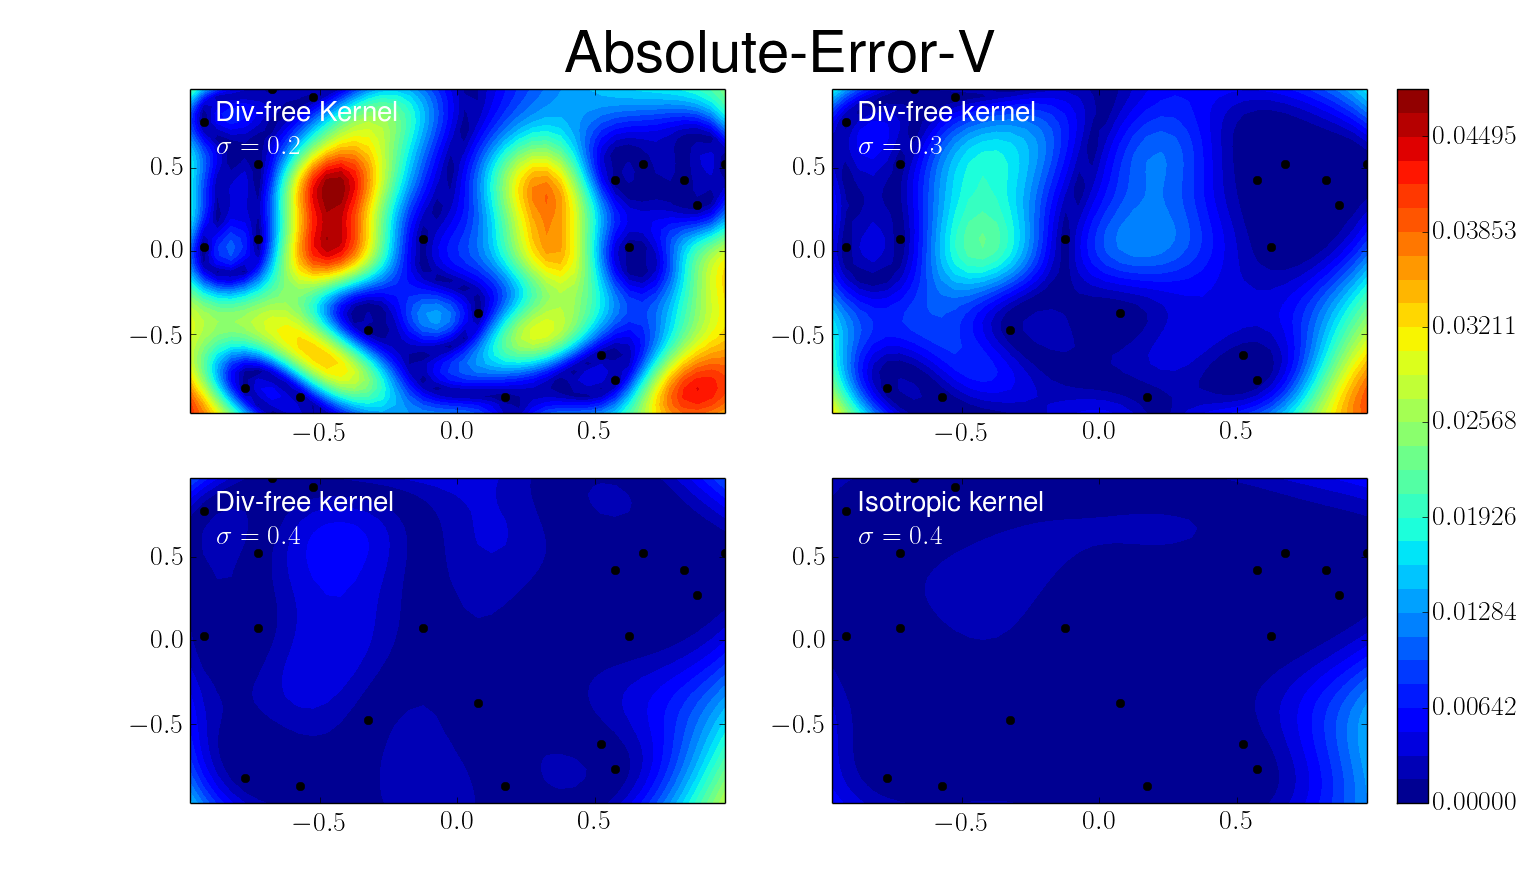
\includegraphics[width=36pc]{plots/Absolute-Error-V-contour.png}
\caption{Same as \ref{contour_u} for the meridional component.  }
\label{contour_v}
\end{figure}

\begin{figure}
\noindent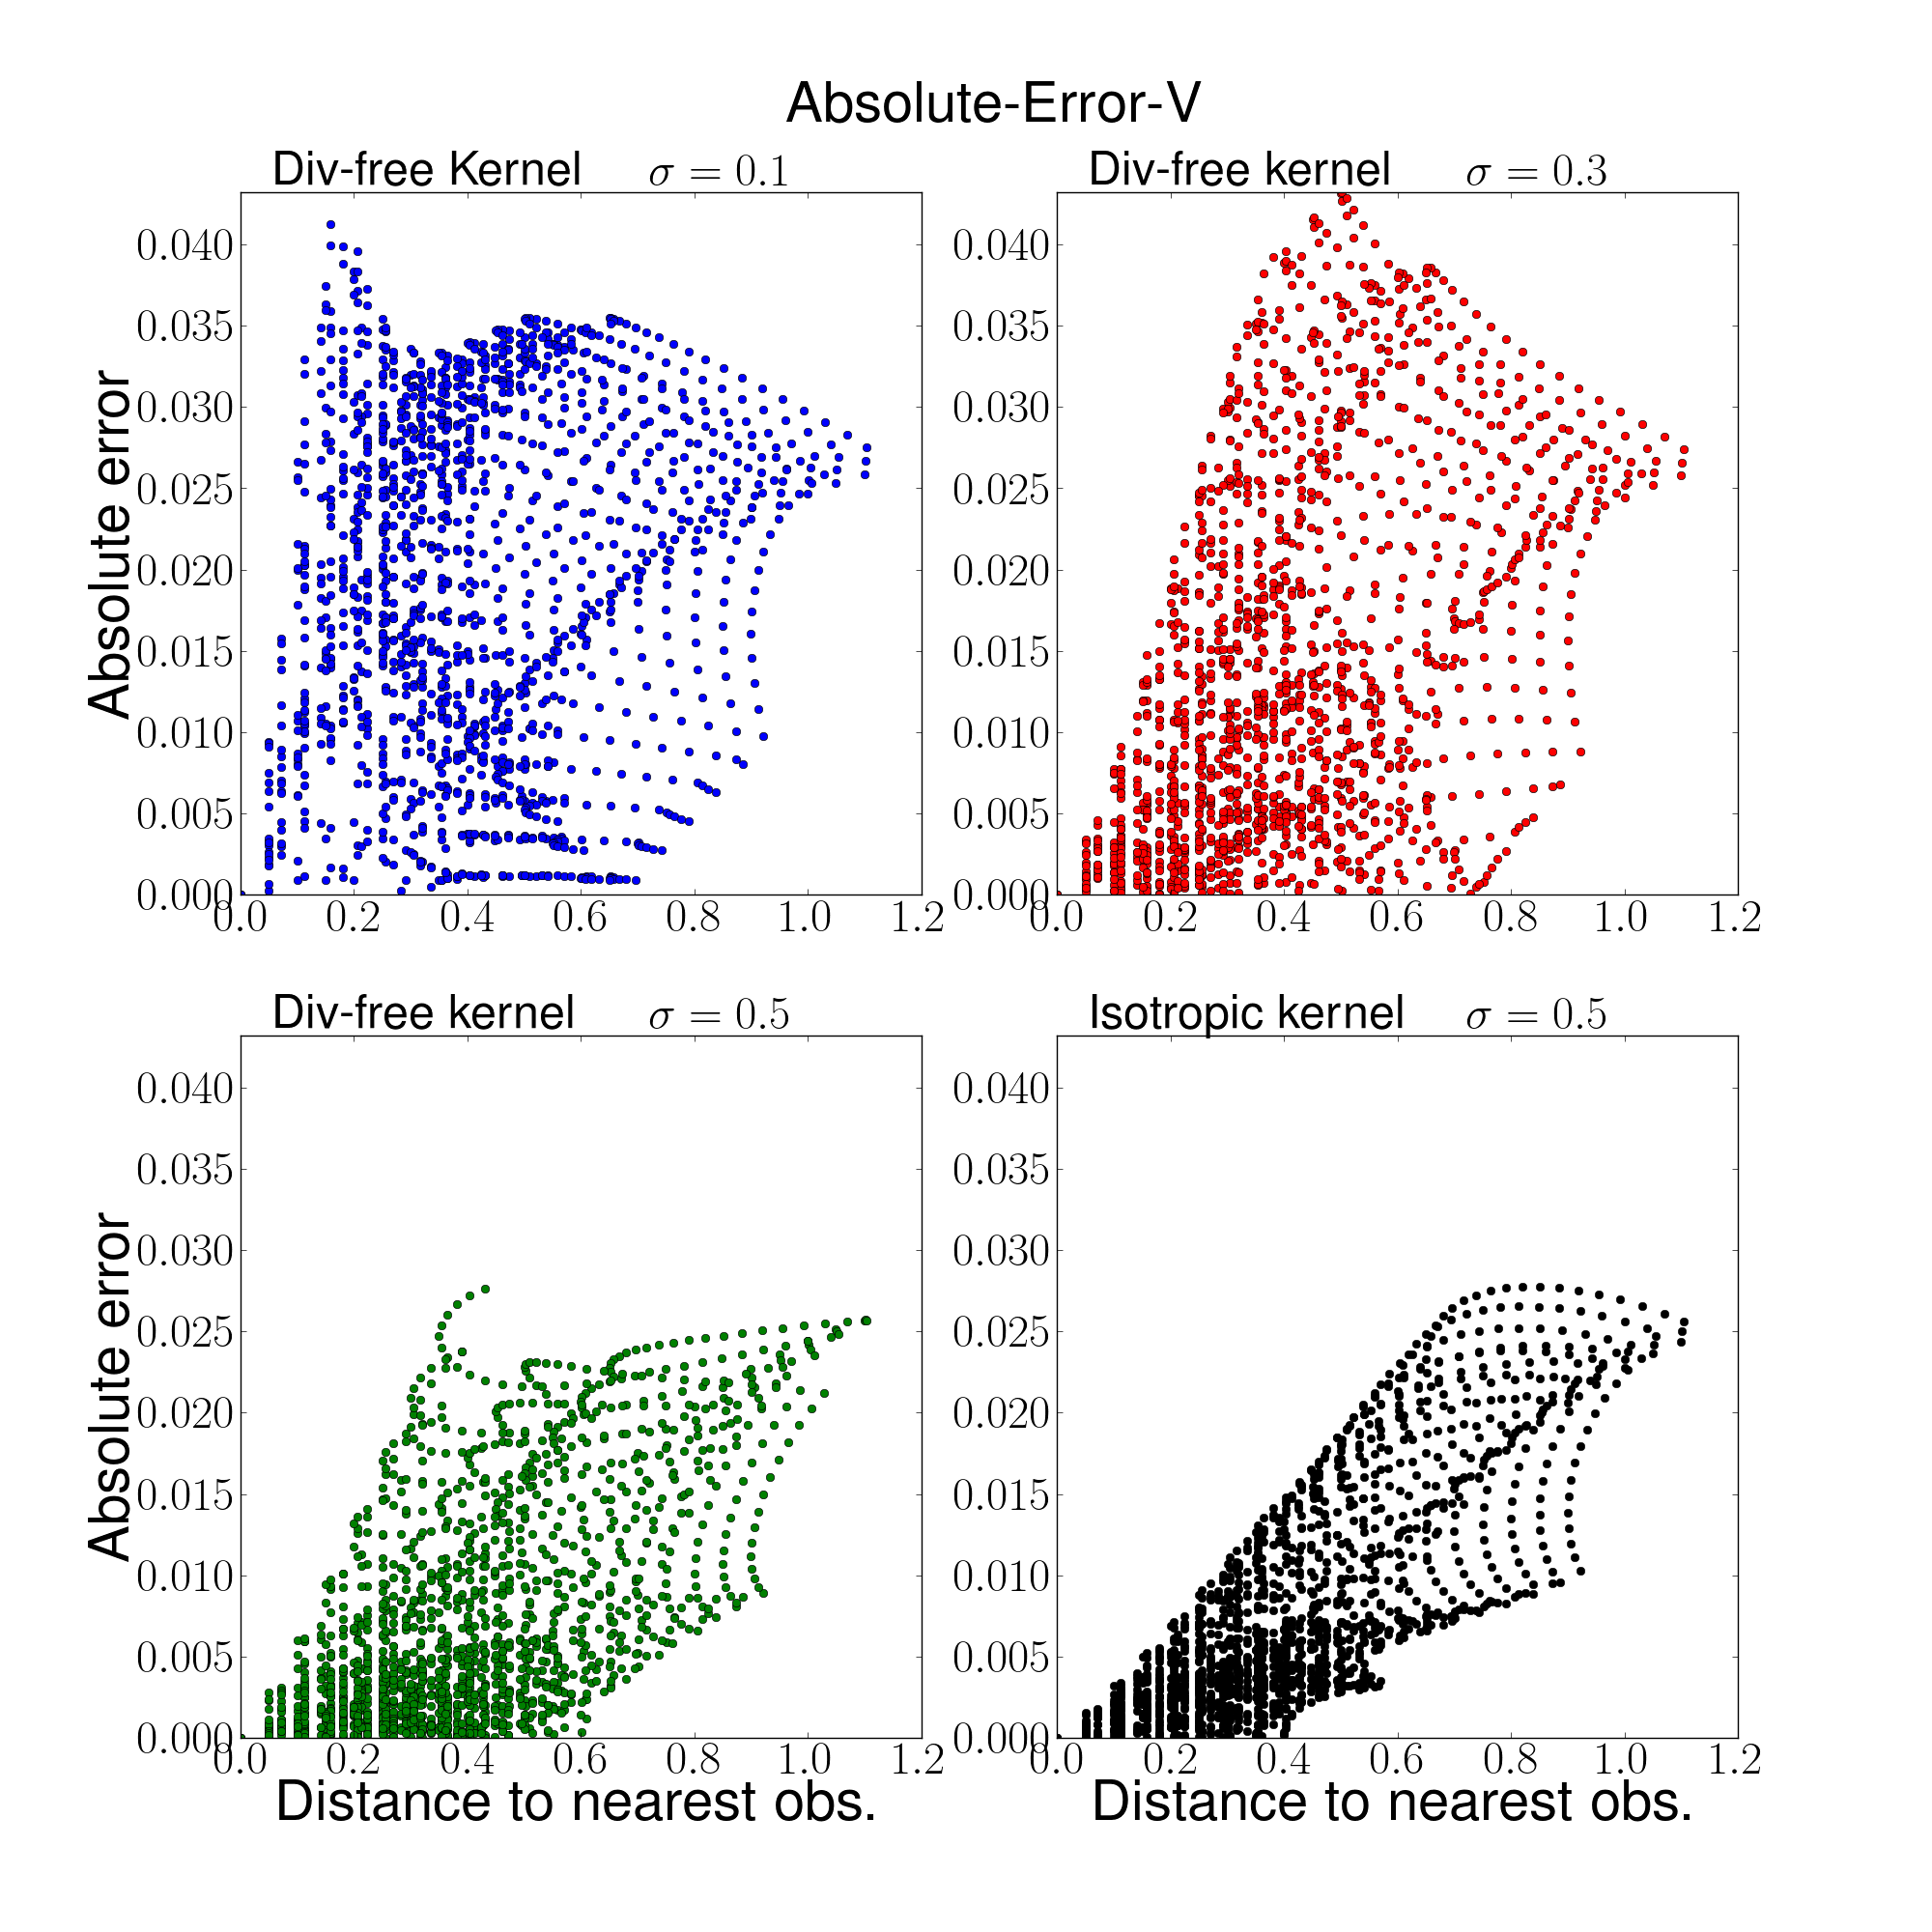
\includegraphics[width=36pc]{plots/Absolute-Error-V-scatter.png}
\caption{Same as Figure \ref{scatter_u} for the meridional component.  }
\label{scatter_v}
\end{figure}

\begin{figure}
\noindent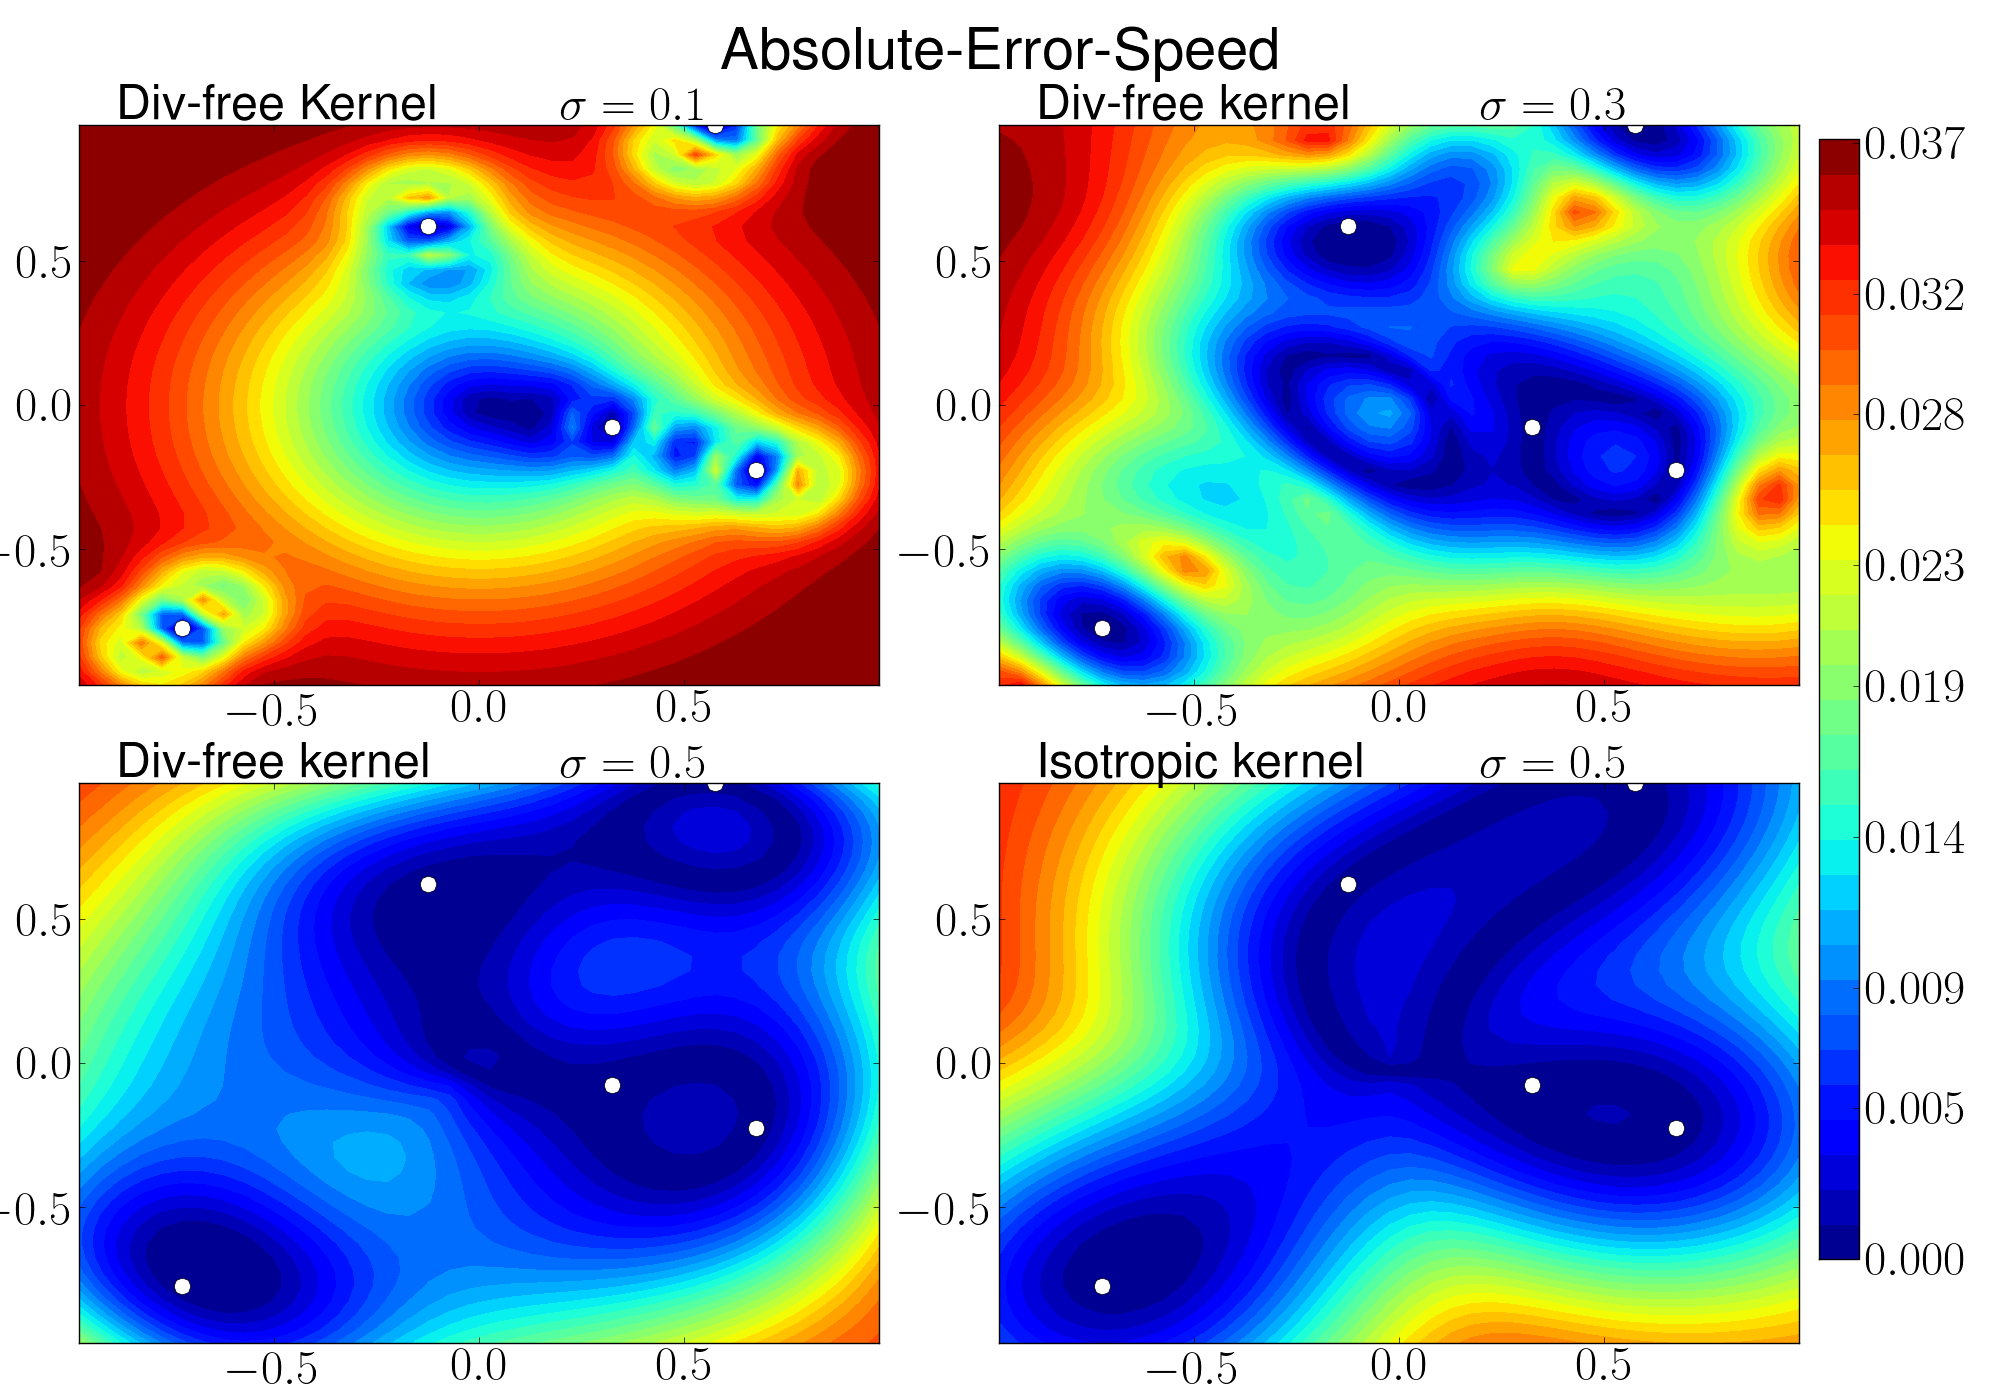
\includegraphics[width=36pc]{plots/Absolute-Error-Speed-contour.png}
\caption{Same as \ref{contour_u} for the absolute velocity. }
\label{contour_speed}
\end{figure}

\begin{figure}
\noindent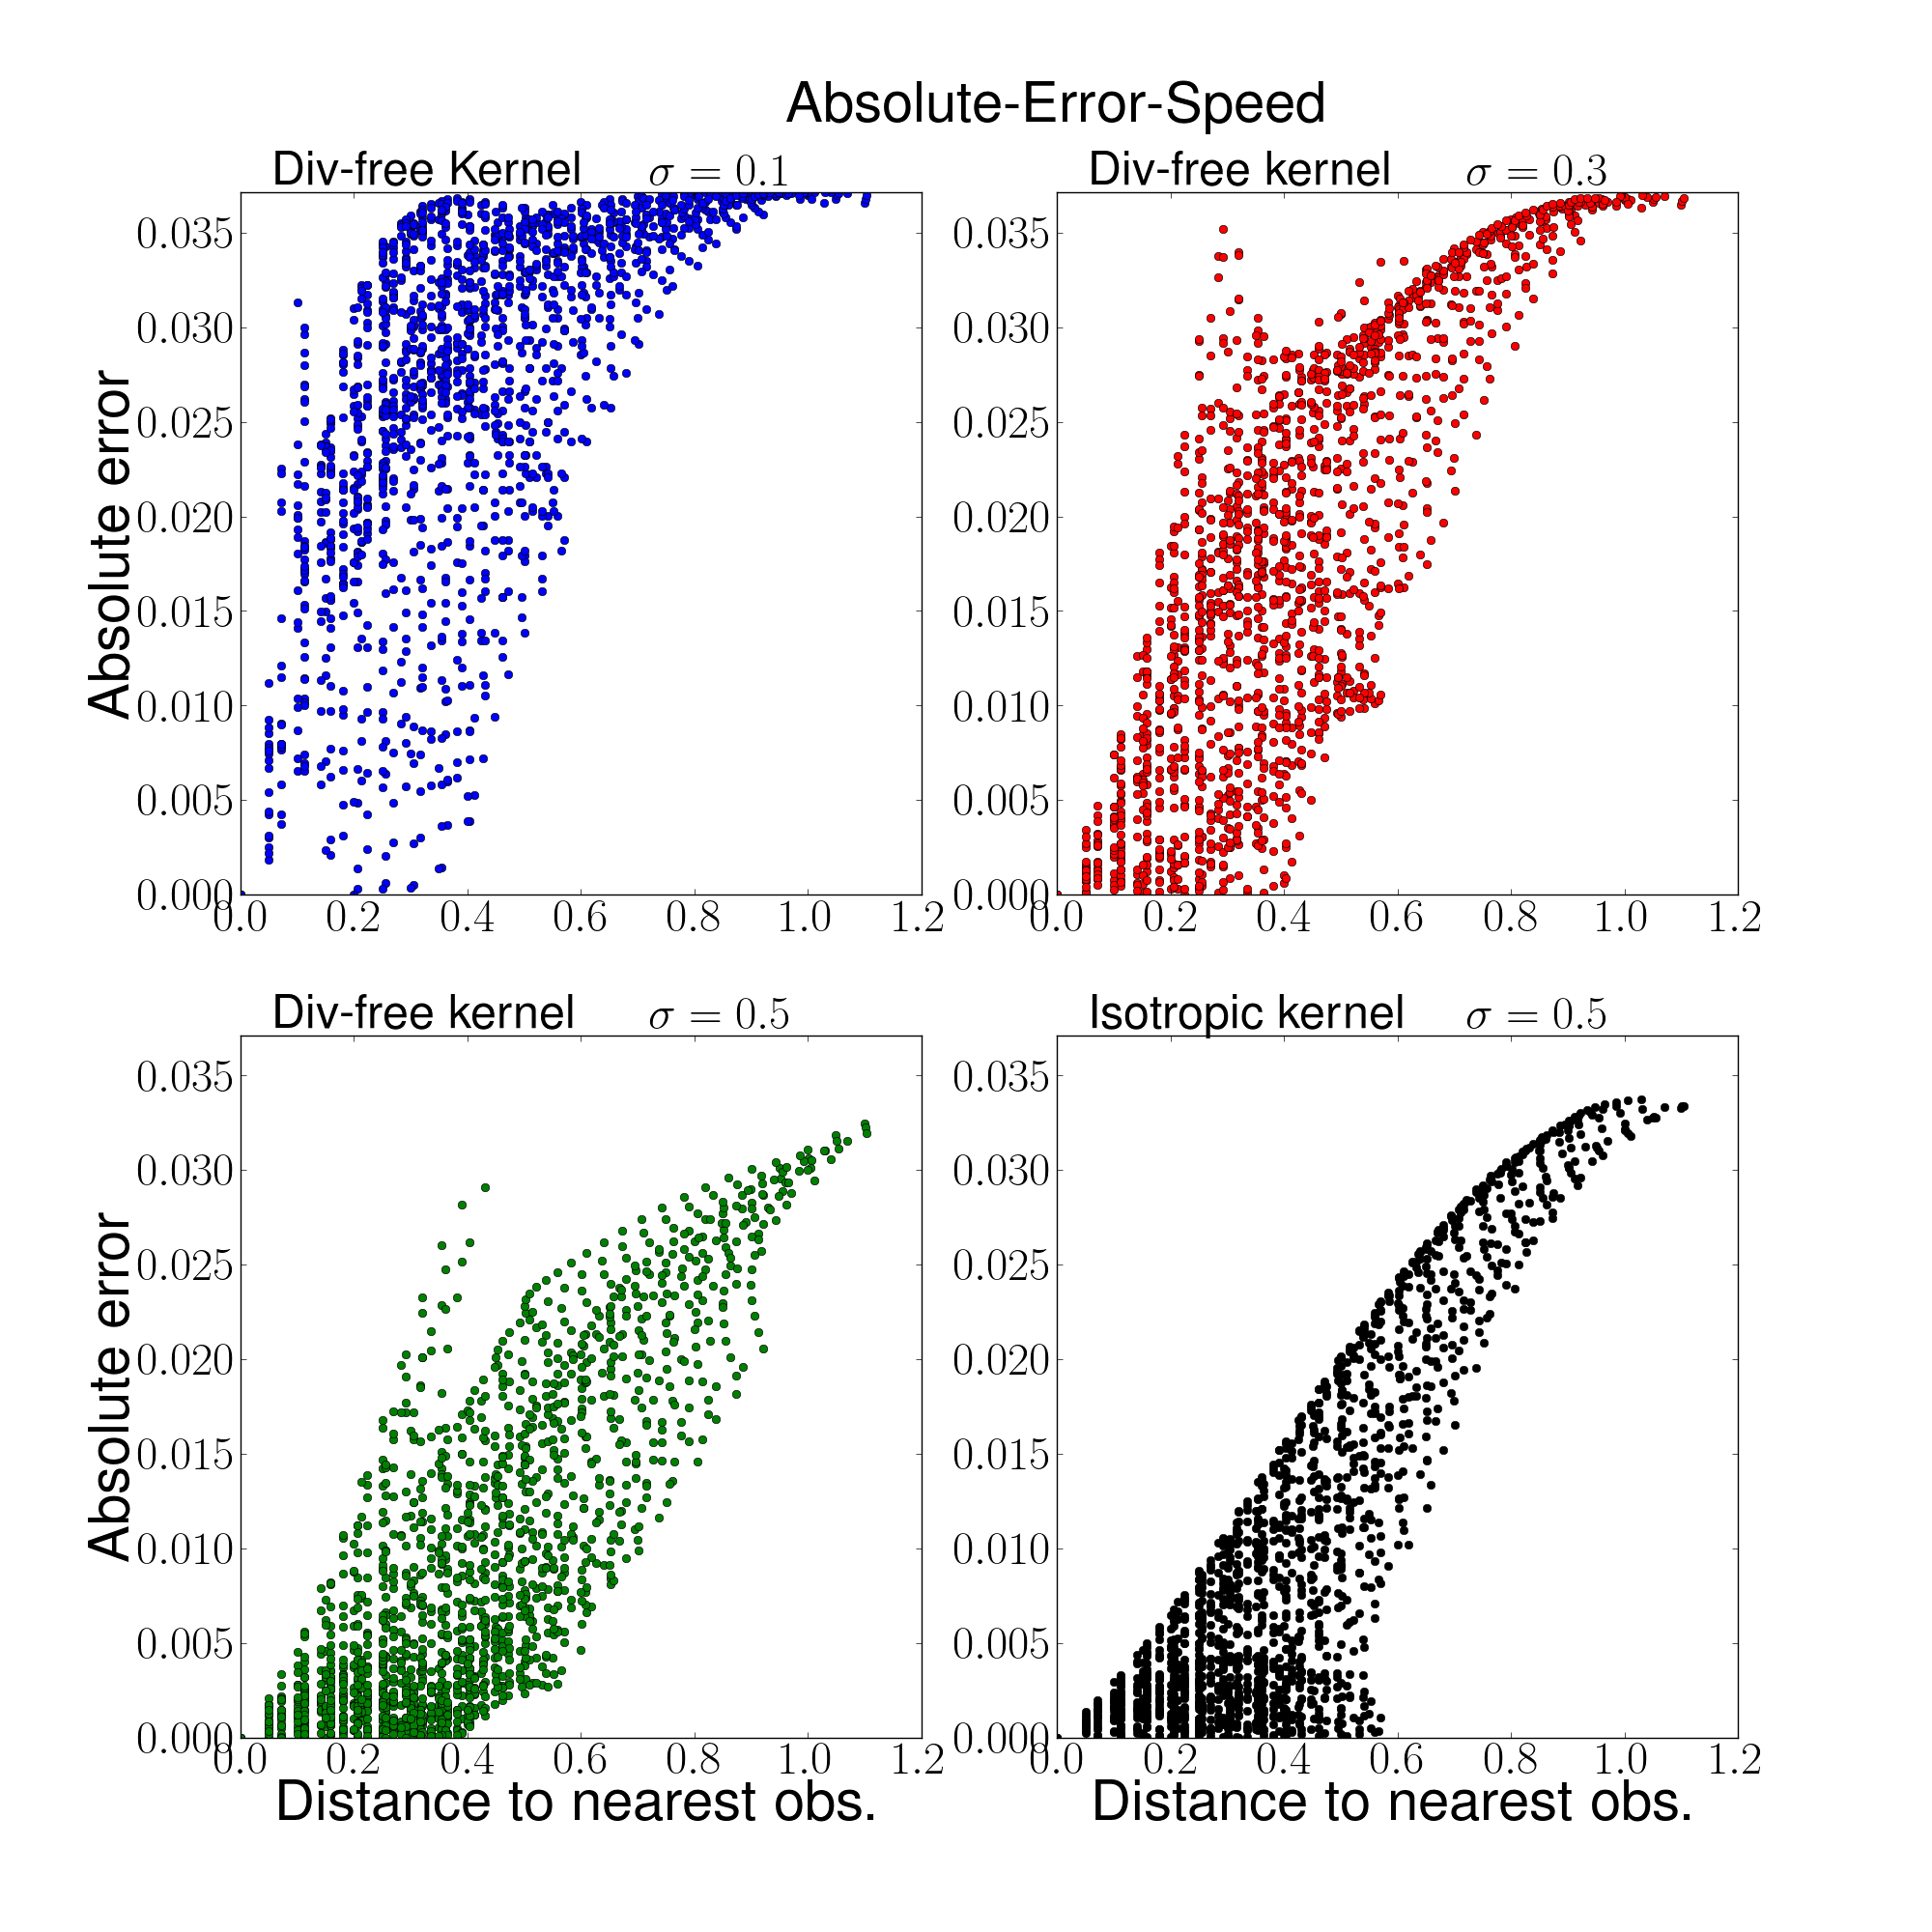
\includegraphics[width=36pc]{plots/Absolute-Error-Speed-scatter.png}
\caption{Same as Figure \ref{scatter_u} for the absolute velocity. }
\label{scatter_speed}
\end{figure}

\begin{figure}
\noindent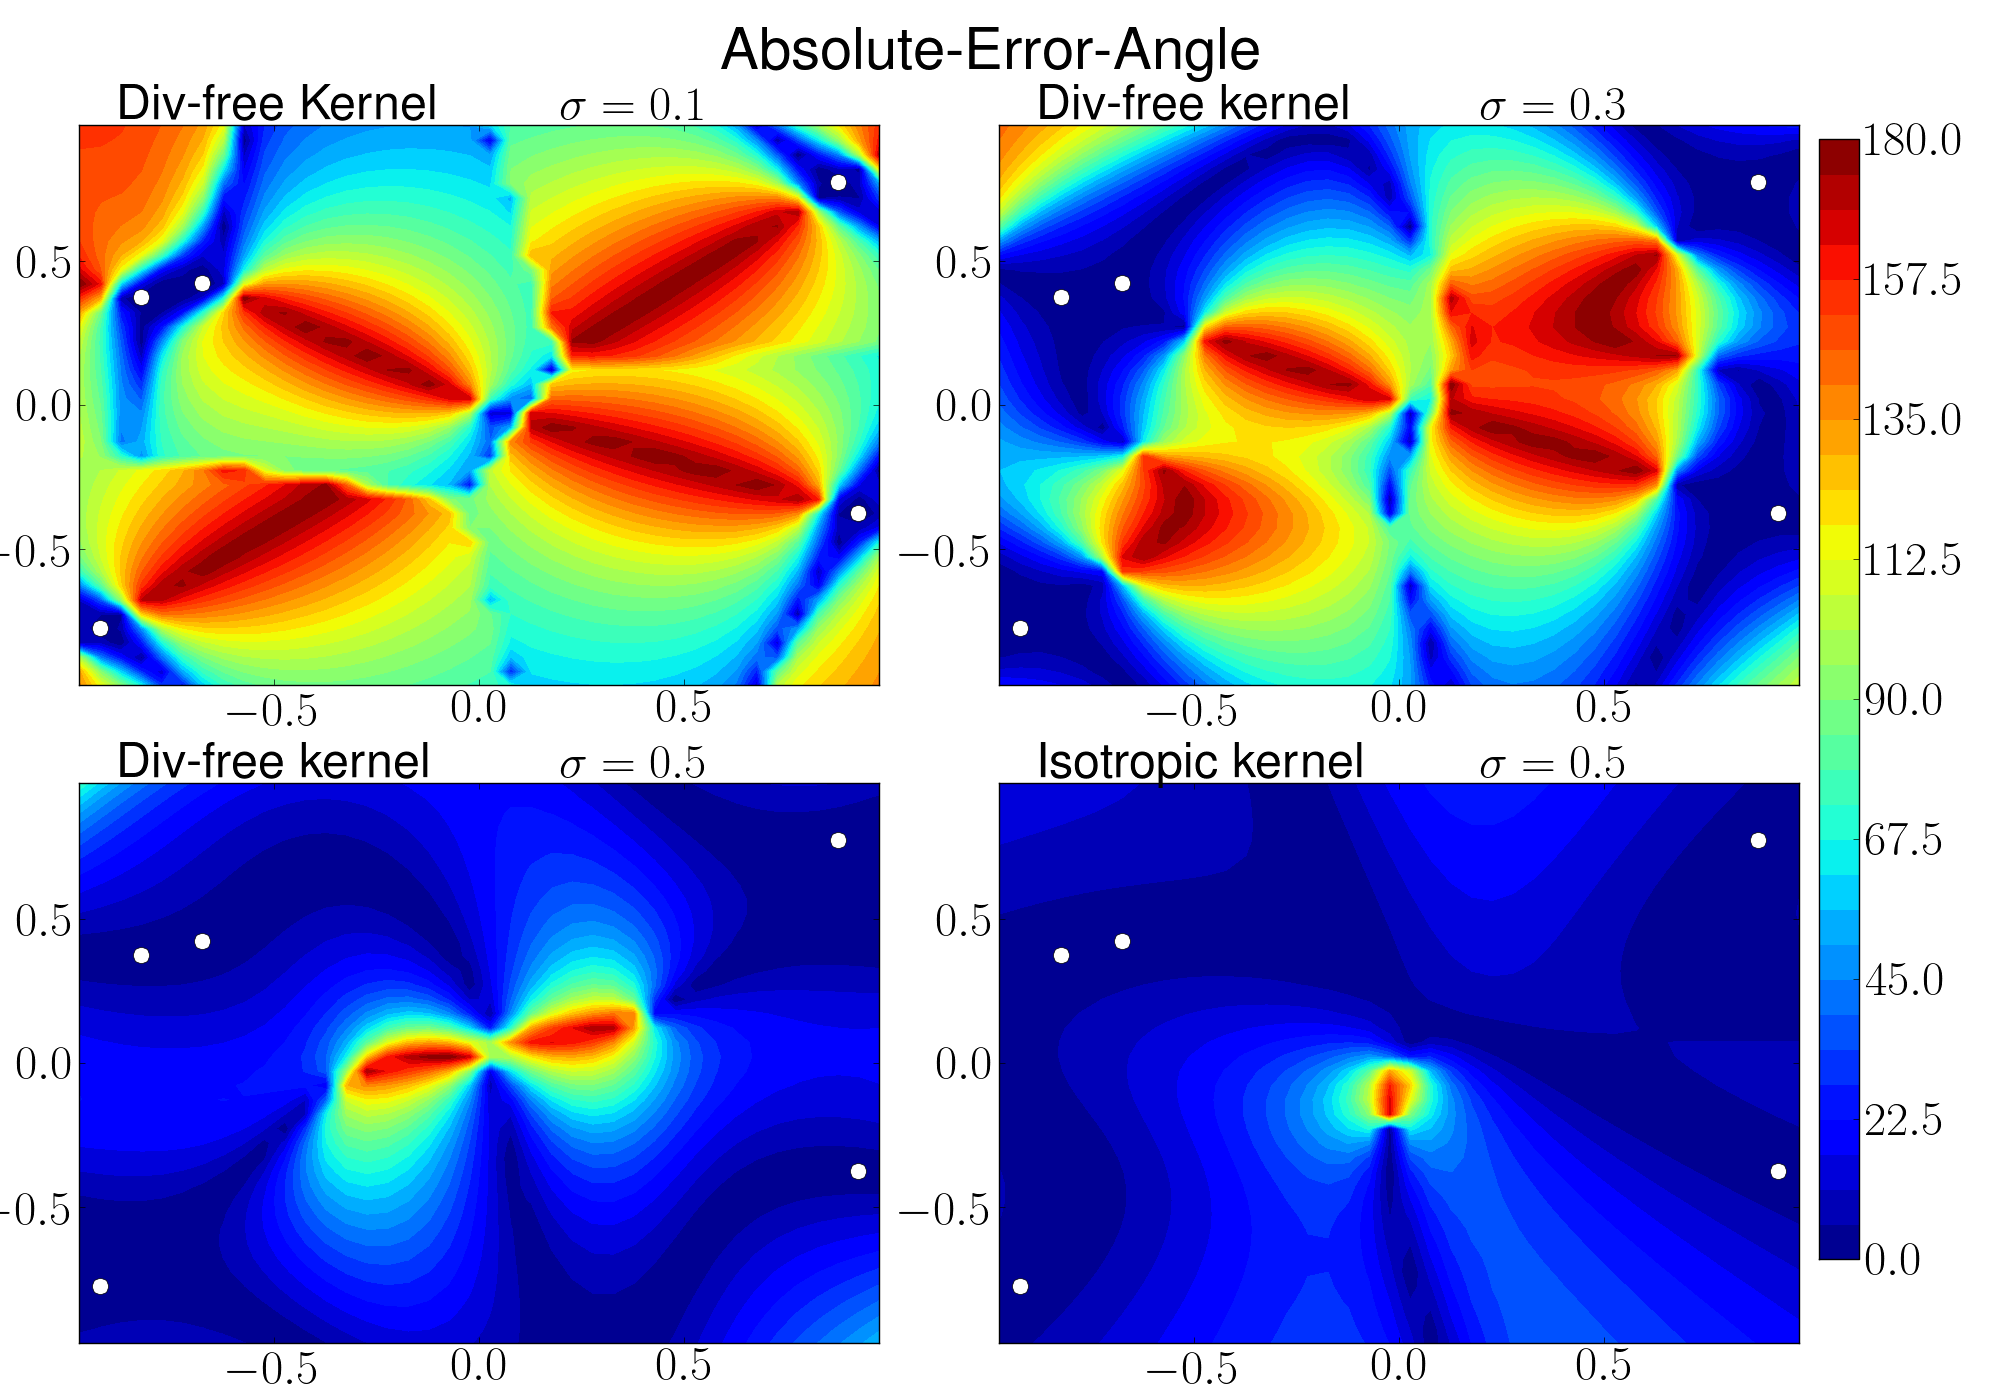
\includegraphics[width=36pc]{plots/Absolute-Error-Angle-contour.png}
\caption{Same as \ref{contour_u} for the azimuth. }
\label{contour_angle}
\end{figure}

\begin{figure}
\noindent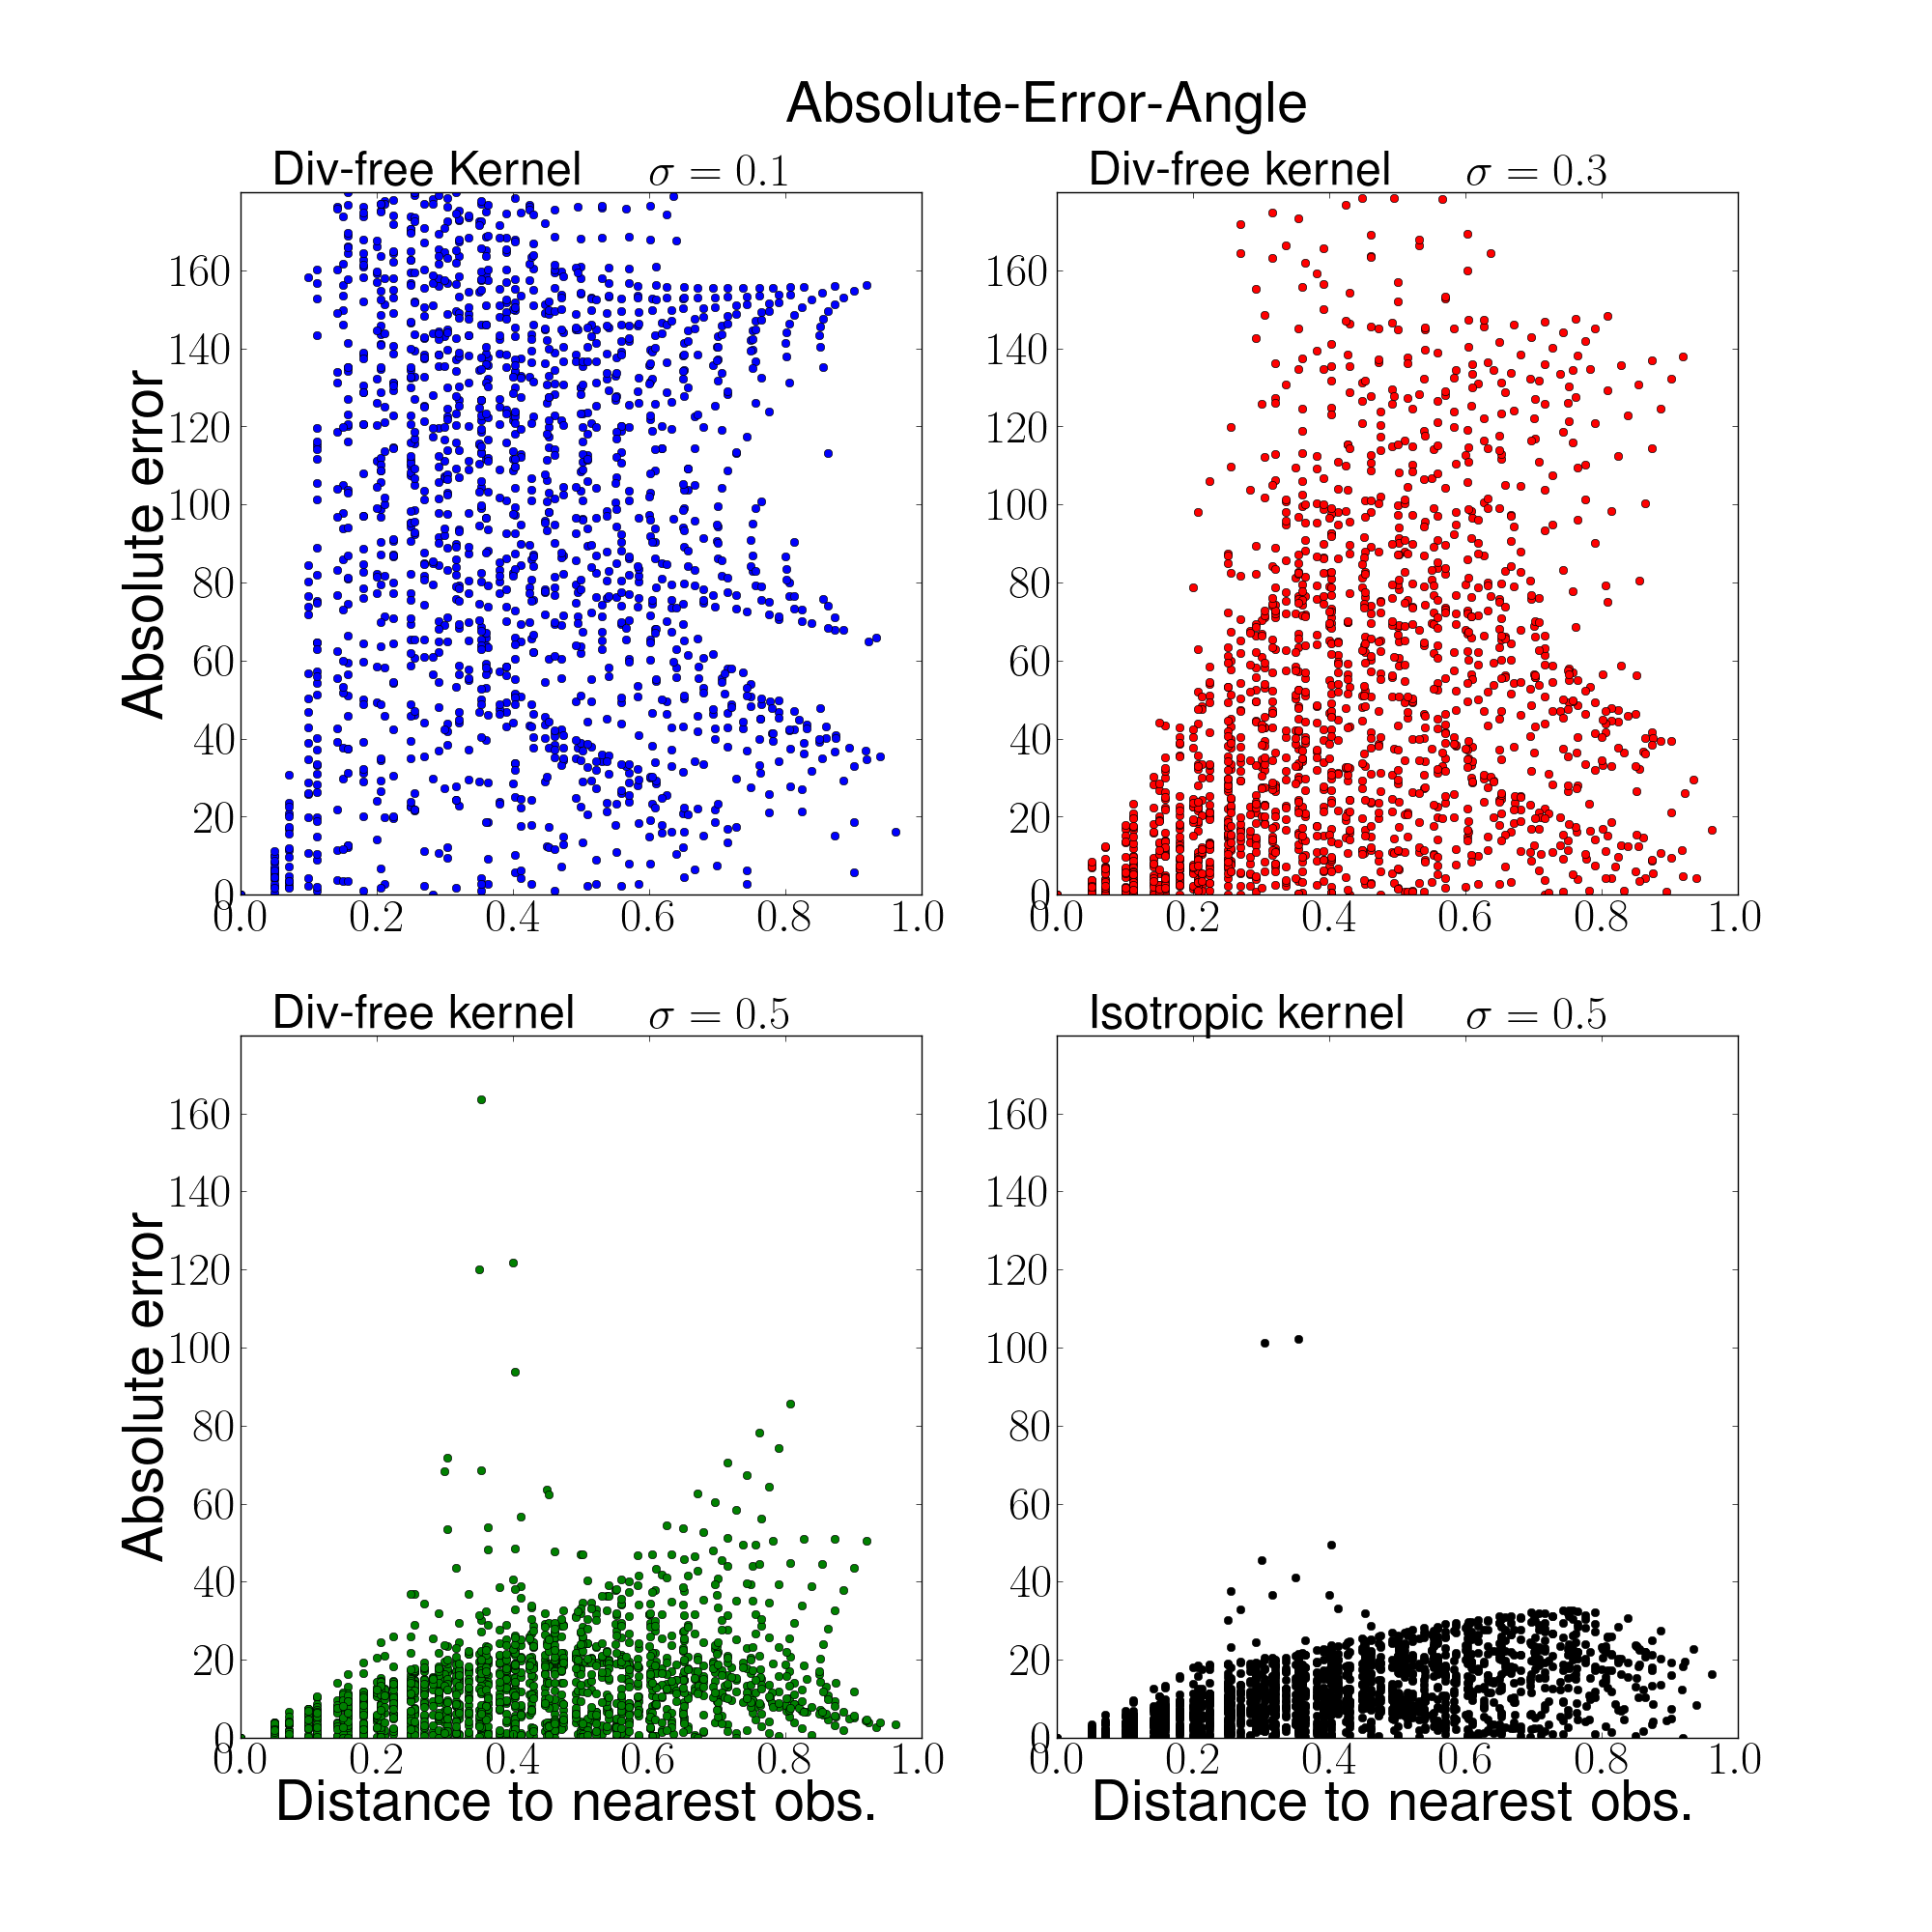
\includegraphics[width=36
pc]{plots/Absolute-Error-Angle-scatter.png}
\caption{Same as Figure \ref{scatter_u} for the azimuth. }
\label{scatter_angle}
\end{figure}

\end{document}